\documentclass[12pt, letterpaper]{article}
\usepackage[utf8]{inputenc}

\hfuzz=1000em
\usepackage[letterpaper, portrait, margin=1in]{geometry}
\usepackage{setspace}
\doublespacing
\usepackage{graphicx}
\usepackage{hyperref}
\usepackage{float}
\usepackage{listings}
\usepackage[format=plain,labelfont={bf,it},textfont=it]{caption}
\makeatletter
\g@addto@macro\@floatboxreset{\centering}
\makeatother

\begin{document}

\begin{titlepage}
    \begin{center}

        \vspace*{5cm}

        \Large{\textbf{L{\"O}VR Demo Docs}}

        \vspace{-0.25cm}

        \Large{\textbf{for Interactive Music Experiences}}

        \vspace{0.5cm}

        \large{assembled by Zachary Talis}

        \vfill

        \small{Spring 2022}

    \end{center}
\end{titlepage}

\tableofcontents
\newpage

\section{Introduction}

\subsection{What does this doc cover?}
We're going to make a monkey spin in L{\"O}VR!\\
L{\"O}VR is a simple-yet-powerful game engine for VR. By the end of this doc, you'll have tackled these L{\"O}VR essentials:
\begin{itemize}
    \item Creating, UV-mapping, and exporting a simple 3D model from Blender.
    \item Slapping some materials onto the model in Substance Painter.
    \item Assembling a final texture in Krita.
    \item Writing a simple Lua script that L{\"O}VR uses to display our model.
\end{itemize}
Parts of this guide are based off L{\"O}VR's "Callbacks and Modules" documentation\footnote{\url{https://lovr.org/docs/Callbacks_and_Modules/}}.

\subsection{Tools we'll use}
You can download everything here for free!\\
\textbf{Blender}\footnote{\url{https://blender.org/}} is a 3D-modelling software that does a little bit of everything.\\
\textbf{Substance Painter}\footnote{\url{https://adobe.com/products/substance3d-painter.html}} is a nondestructive, mask-based, Adobe-owned texturing tool. It's free with an \verb|edu| email address.\\
\textbf{Krita}\footnote{\url{https://krita.org/}} is an image manipulation and painting tool.\\
\textbf{L{\"O}VR}\footnote{\url{https://lovr.org/}} is a cross-platform VR engine that flouts intuitive Lua scripting and a light footprint.

\section{Blender (Suzanneification)}

\subsection{A fresh Suzanne}
\begin{enumerate}
    \item Make a new Blender file, delete any default objects, and add a \verb|Mesh > Monkey|. Say hello to our new friend Suzanne\footnote{\url{https://docs.blender.org/manual/en/latest/modeling/meshes/primitives.htm\#monkey}}!
    \item Go into \verb|Edit Mode|.
    \item Unwrap some UVs for our Suzanne. You've got two options: either \verb|Smart UV Project| or marking the UV seams yourself.
          \begin{figure}[H]
              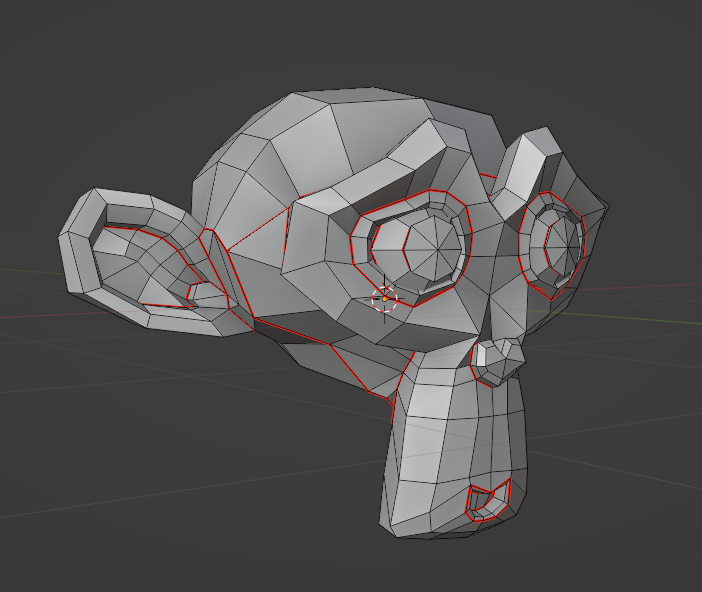
\includegraphics[scale=0.5]{assets/img/blender-seams.png}
              \caption{UV seams marked on Suzanne.}
          \end{figure}
\end{enumerate}

\subsection{Exporting to glTF}
\begin{enumerate}
    \item \verb|File > Export > glTF 2.0|.
    \item Change the \verb|Format| to \verb|glTF Embedded (.gltf)|, and export.
\end{enumerate}

\section{Substance Painter}

\subsection{New file}
\begin{enumerate}
    \item \verb|File > New|, as all great things begin.
    \item \verb|Template|: set to \verb|PBR - Metallic Roughness Alpha-blend|.
    \item \verb|File|: select your exported glTF.
    \item \verb|Project Settings|: \verb|Document Resolution| of 2048.
    \item Make sure \verb|Auto-unwrap| is disabled, then press \verb|OK|.
\end{enumerate}

\subsection{Rendering maps}
\begin{enumerate}
    \item \verb|Edit > Bake Mesh Maps|.
    \item Set \verb|Output Size| to 2048, then \verb|Bake selected textures|.
\end{enumerate}

\subsection{Smart materials}
\begin{enumerate}
    \item Search the assets browser for smart materials of your choosing. Drop 'em onto Suzanne.
    \item For each smart material layer, create a black mask.
    \item For each mask, use \verb|Polygon Fill > UV chunk fill| to give Suzanne some pizzazz.
          \begin{figure}[H]
              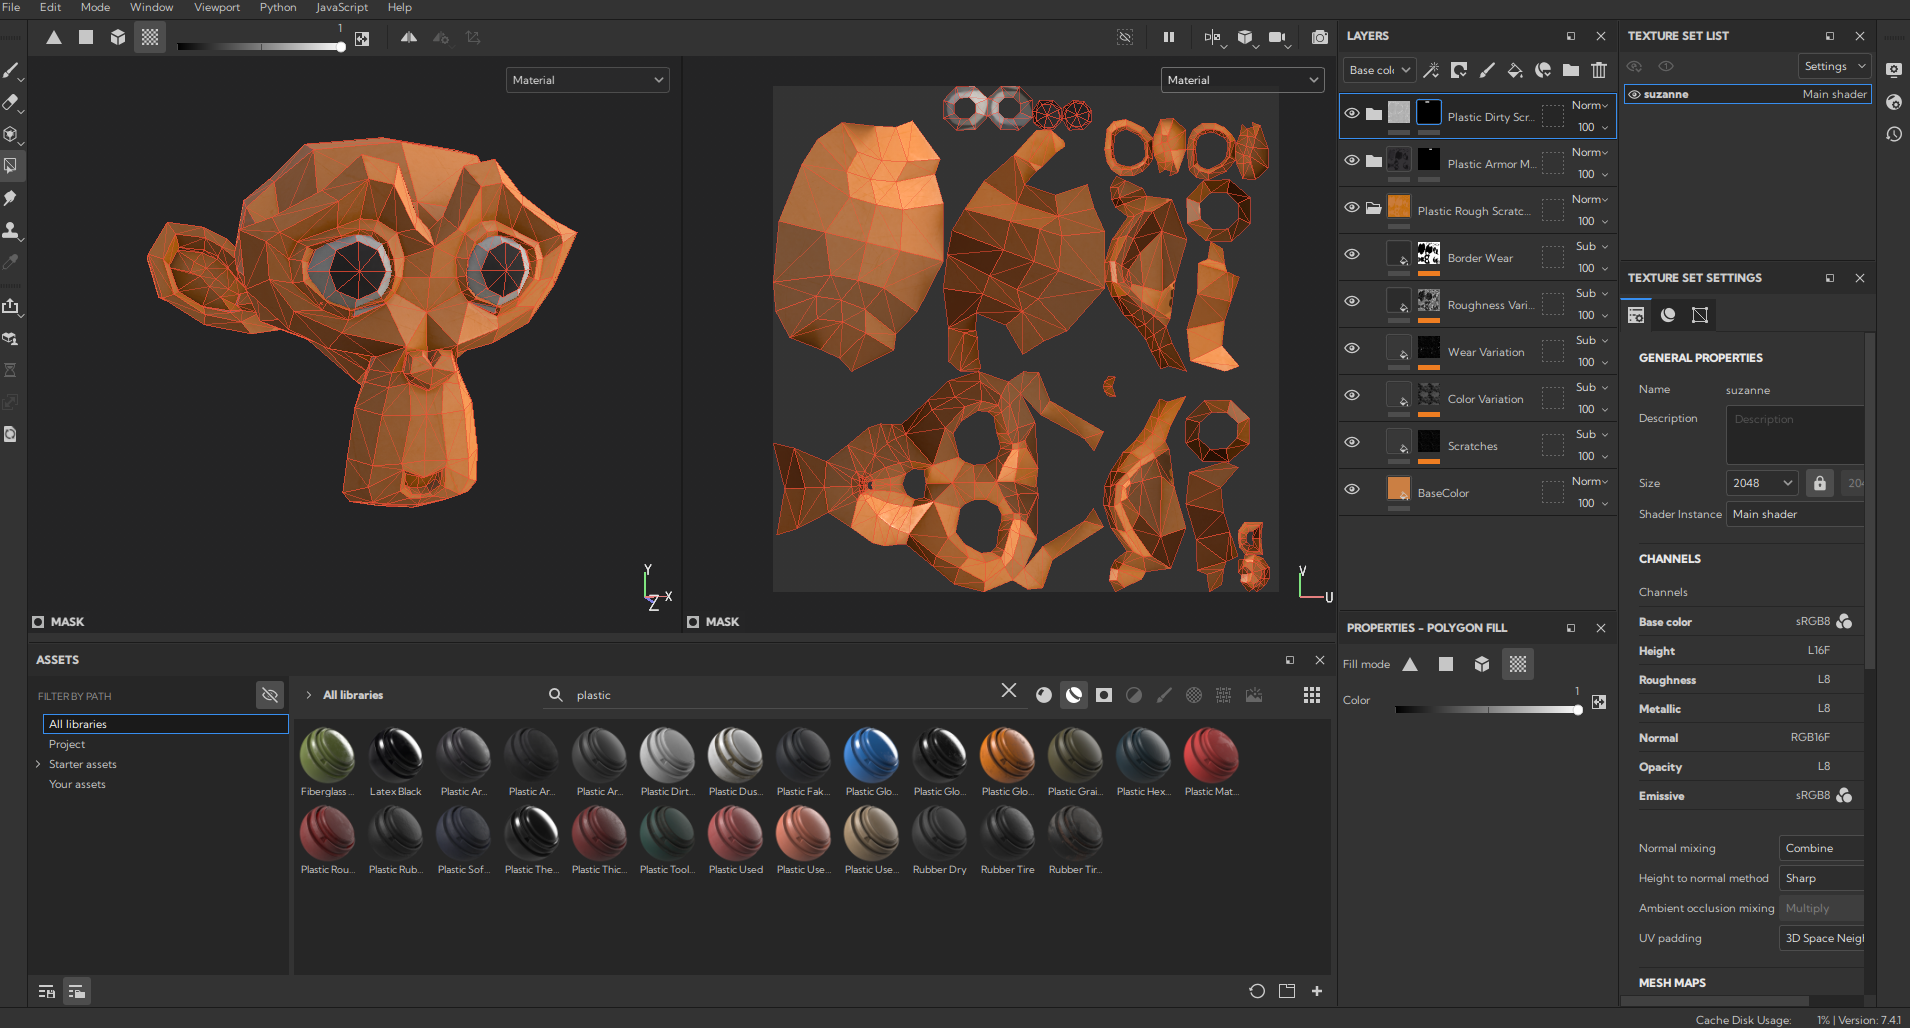
\includegraphics[scale=0.4]{assets/img/substance-project.png}
              \caption{Substance Painter project with decked-out Suzanne.}
          \end{figure}
\end{enumerate}

\subsection{Exporting}
\begin{enumerate}
    \item \verb|File > Export Textures...|.
    \item Export using both the \verb|PBR Metallic Roughness| and \verb|Mesh Maps| templates.
\end{enumerate}

\section{Krita}

\subsection{An ambient excursion}
\begin{enumerate}
    \item Open the \verb|ambient_occlusion| and \verb|BaseColor| images in Krita. Plop them onto two separate layers (ambient occlusion on top).
    \item Set the ambient occlusion layer to a low opacity and the \verb|Addition| blending mode.
    \item \verb|File > Export|, then save as a PNG.
          \begin{figure}[H]
              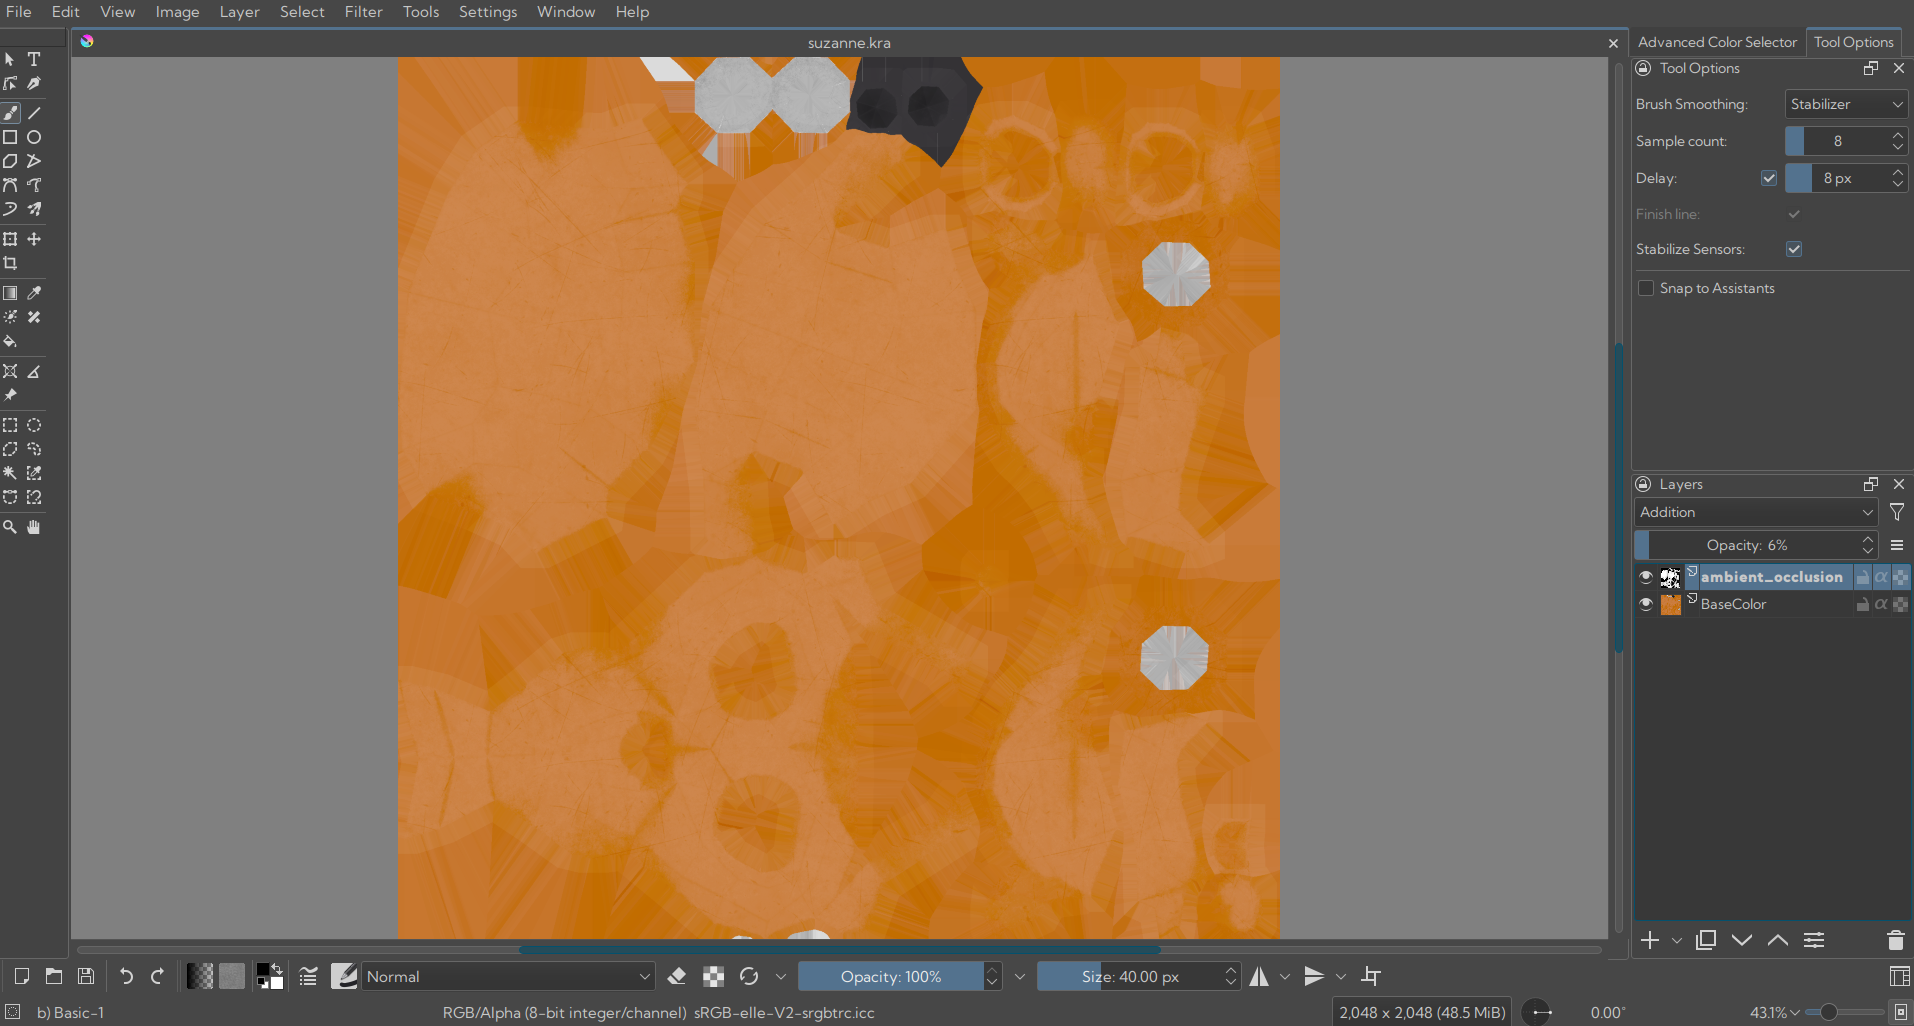
\includegraphics[scale=0.4]{assets/img/krita-project.png}
              \caption{Krita project with those two texture layers.}
          \end{figure}
\end{enumerate}

\section{Blender (Final Export)}

\subsection{Giving Suzanne our texture}
TK\\
Then export again.
\begin{enumerate}
    \item Give Suzanne a new material.
    \item Configure Suzanne's material with the texture PNG as shown below in \textbf{Figure 4}.
    \item Export to glTF once again.
          \begin{figure}[H]
              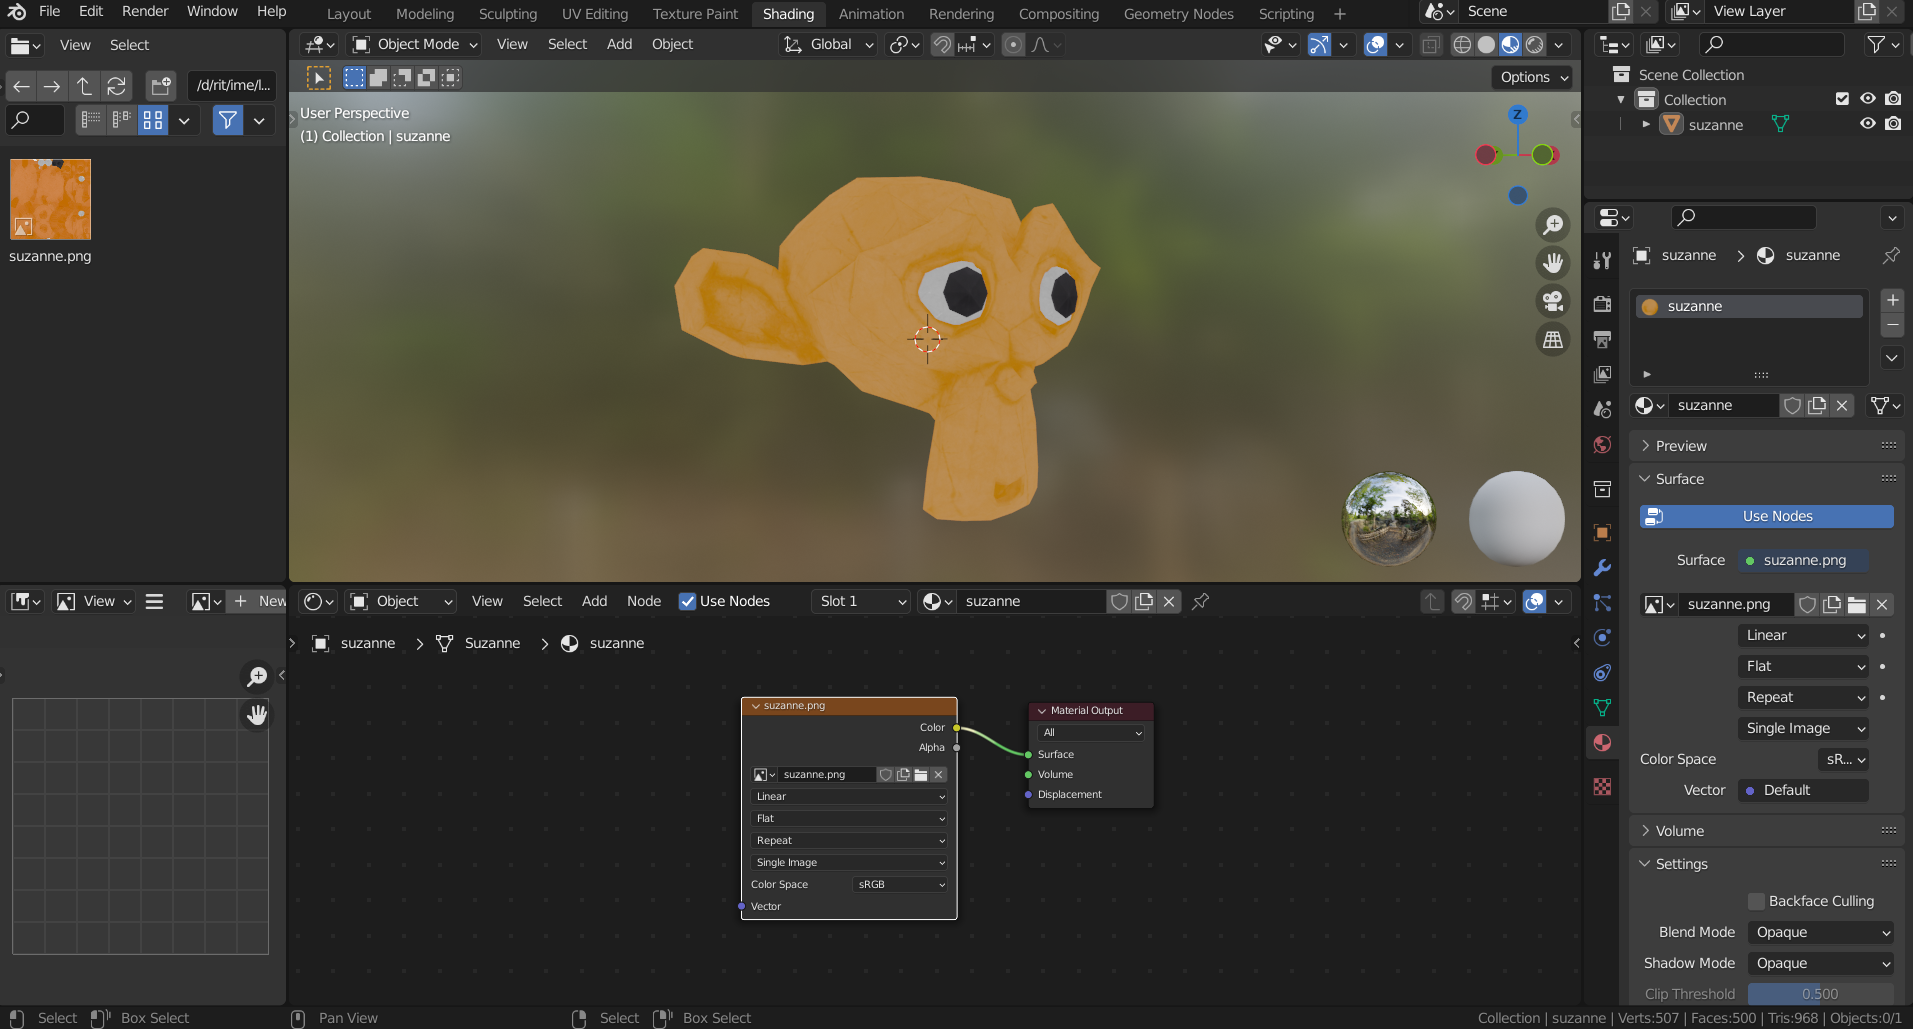
\includegraphics[scale=0.4]{assets/img/blender-material.png}
              \caption{Blender project showcasing Suzanne's nifty material nodes.}
          \end{figure}
\end{enumerate}

\section{L{\"O}VR}

\subsection{Project structure}
\begin{enumerate}
    \item Create a folder on your computer that contains:
          \begin{enumerate}
              \item A subfolder \verb|assets| with subsubfolder \verb|gltf|. Place your exported model inside here.
              \item Empty text files \verb|conf.lua| and \verb|main.lua|.
              \item L{\"O}VR's executable/dependencies from the L{\"O}VR download page\footnote{\url{https://lovr.org/downloads/}}.
          \end{enumerate}
    \item Open the directory in a text editor. Visual Studio Code\footnote{\url{https://code.visualstudio.com/}} works great for this purpose.
\end{enumerate}

\subsection{conf.lua, for convenience's sake}
To force L{\"O}VR to run in desktop mode (rather than in VR mode), add the following code to \verb|conf.lua|:
\begin{center}
    \begin{tabular}{c}
        \begin{lstlisting}[language={[5.2]Lua},basicstyle=\footnotesize]
        function lovr.conf(t)
            t.modules.headset = false
        end
        \end{lstlisting}
    \end{tabular}
\end{center}

\subsection{Resource imports}
Drop this code into \verb|main.lua| to import Suzanne's model:
\begin{center}
    \begin{tabular}{c}
        \begin{lstlisting}[language={[5.2]Lua},basicstyle=\footnotesize]
        function lovr.load()
            suzanne = lovr.graphics.newModel("assets/gltf/suzanne.gltf")
        end
        \end{lstlisting}
    \end{tabular}
\end{center}

\subsection{Spinny Suzanne}
Add some more code to \verb|main.lua| to make Suzanne appear (and spin)!
\begin{center}
    \begin{tabular}{c}
        \begin{lstlisting}[language={[5.2]Lua},basicstyle=\footnotesize]
        function lovr.draw()
            suzanne:draw(0, 0, -3, 1, lovr.timer.getTime())
        end
        \end{lstlisting}
    \end{tabular}
\end{center}

\subsection{Running the project}
From command line, run L{\"O}VR's executable with the current directory as its sole argument. On Linux, this looks like:
\begin{center}
    \begin{tabular}{c}
        \begin{lstlisting}[language=Bash,basicstyle=\footnotesize]
            ./lovr-x86_64.AppImage .
        \end{lstlisting}
    \end{tabular}
\end{center}
You should see spinny Suzanne!

\begin{figure}[H]
    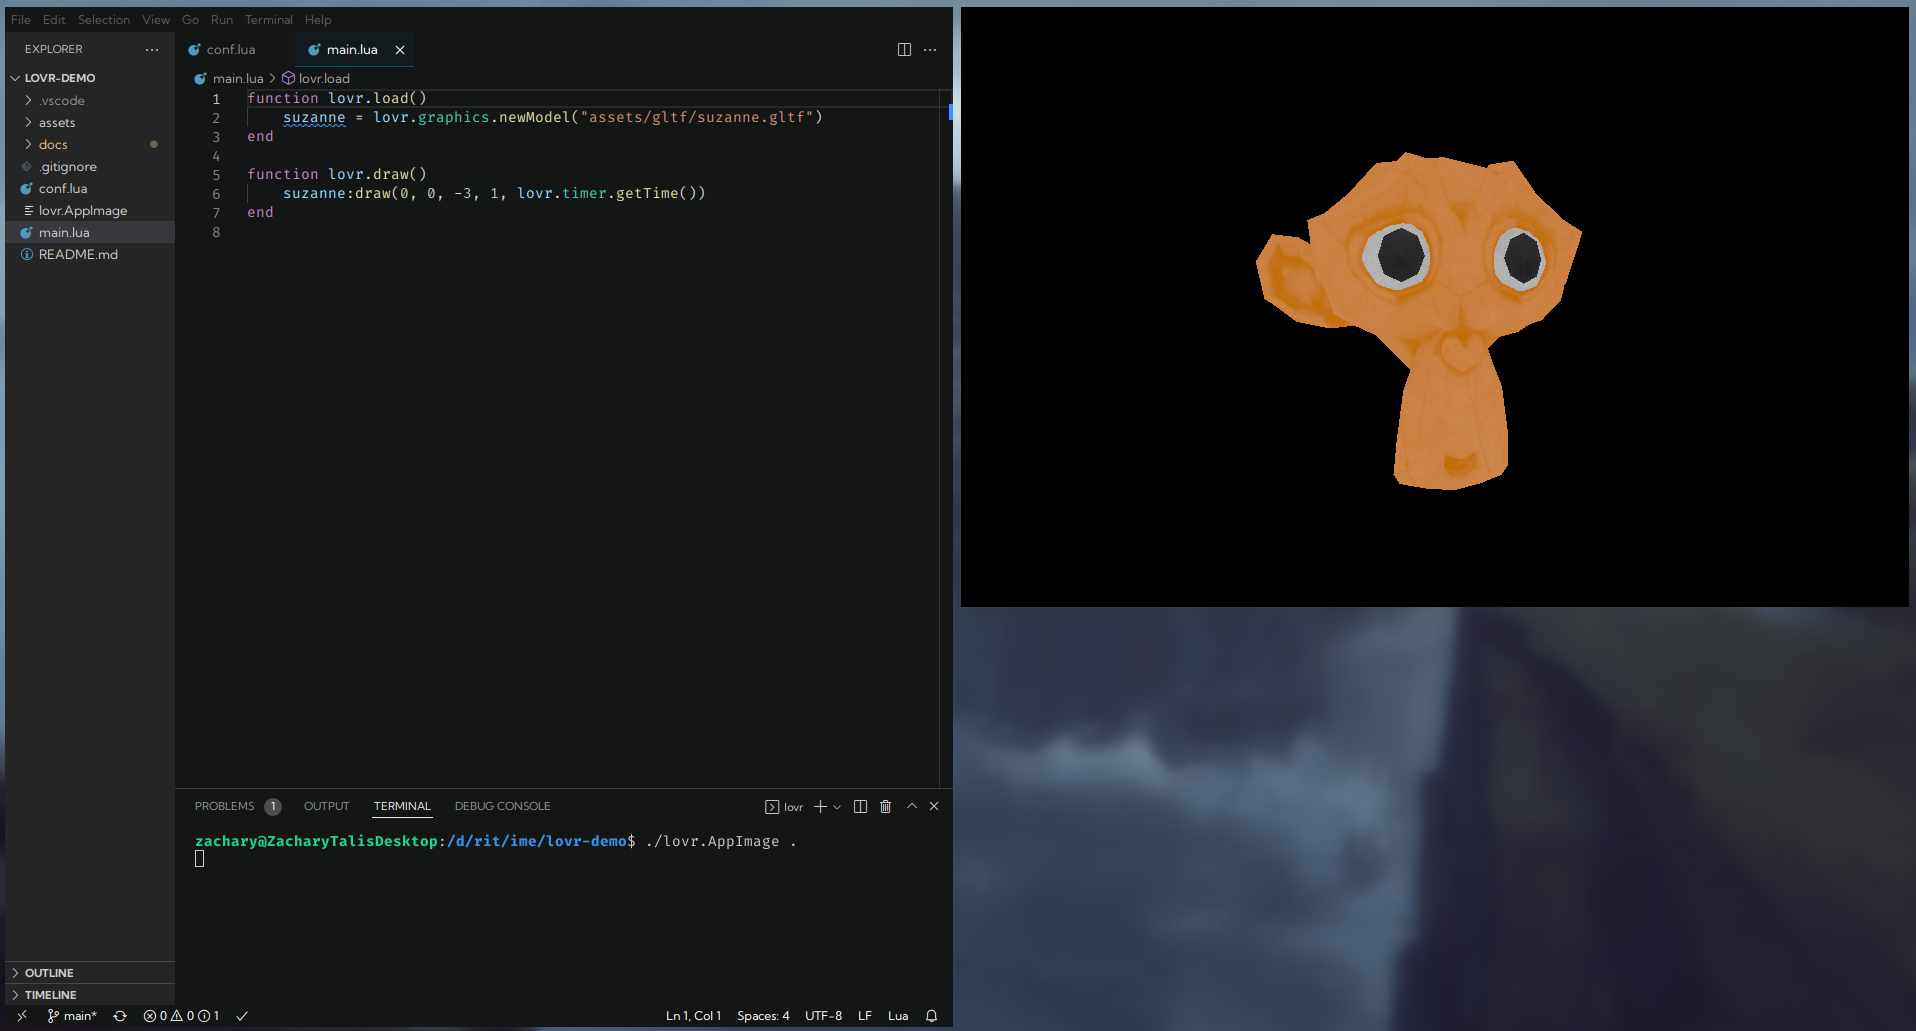
\includegraphics[scale=0.4]{assets/img/lovr-project.png}
    \caption{L{\"O}VR project running and open in Visual Studio Code.}
\end{figure}

\end{document}